\subsection{Introduction}

In the realm of machine learning, decision trees have emerged as a potent tool for both classification and regression tasks, owing to their intuitive decision-making process and ease of interpretation. The basic principle behind decision trees is to split the data into subsets based on the values of input features, thus creating a tree-like model of decisions, as illustrated in Fig.~\ref{fig:tree_scheme}. This methodology is highly effective for data mining applications and has been a subject of extensive research across various disciplines such as statistics, machine learning, and data mining.

% \subsubsection{Ensemble Learning: From Random Forests to Gradient Boosting}

\begin{figure}[htpb]
   \centering
    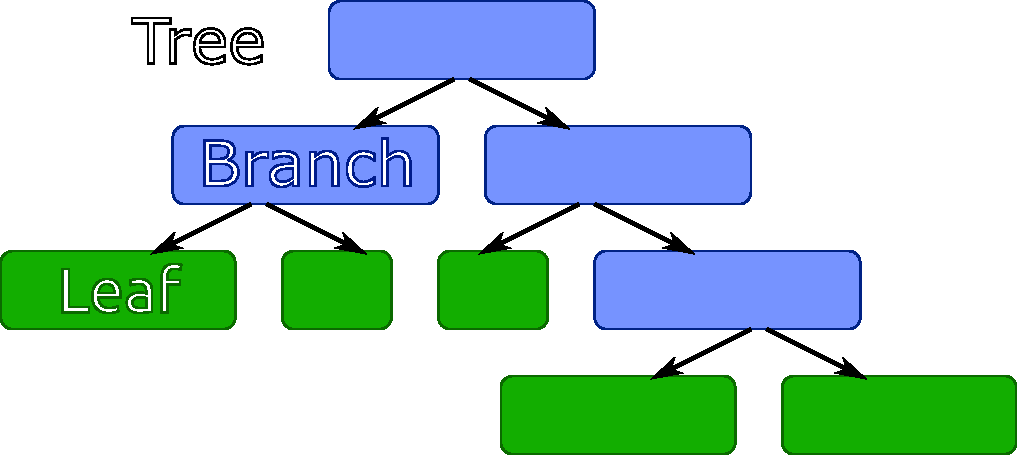
\includegraphics[width=0.5\linewidth]{images/boost/tree_scheme.pdf}
    \caption{One desicion tree - weak learner.}
    \label{fig:tree_scheme}
\end{figure}


Decision trees are a class of algorithms employed for both classification and regression tasks. They have gained popularity due to their ease of interpretation and resemblance to human decision-making processes~\cite{kotsiantis2013decision, song2015decision}. The methodology behind decision trees involves creating a tree-like model (see Fig.~\ref{fig:tree_scheme}) of decisions based on the values of input features, which is particularly effective for data mining applications~\cite{song2015decision}. 
One of the notable advancements in decision tree algorithms came with Ross Quinlan's development of ID3 and its improved version C4.5, which extended the capability to handle both categorical and numerical features through the use of 
% information gain ratio (IGR) 
\acrfull{igr} (see~\cite{mienye2019prediction} for information).

Building upon the foundation laid by decision trees, ensemble learning techniques like 
% Random Forests (RF)
\acrfull{rf}
and Gradient Boosting (GB) have been developed to tackle more complex problems. Random Forests extend the decision tree concept by constructing a 'forest' of decision trees, each trained on a random subset of the data and features. The ensemble's final prediction is an aggregation of the predictions from individual trees, significantly reducing variance compared to a single decision tree, and often achieving higher accuracy.

\begin{figure}[ht]
   \centering
    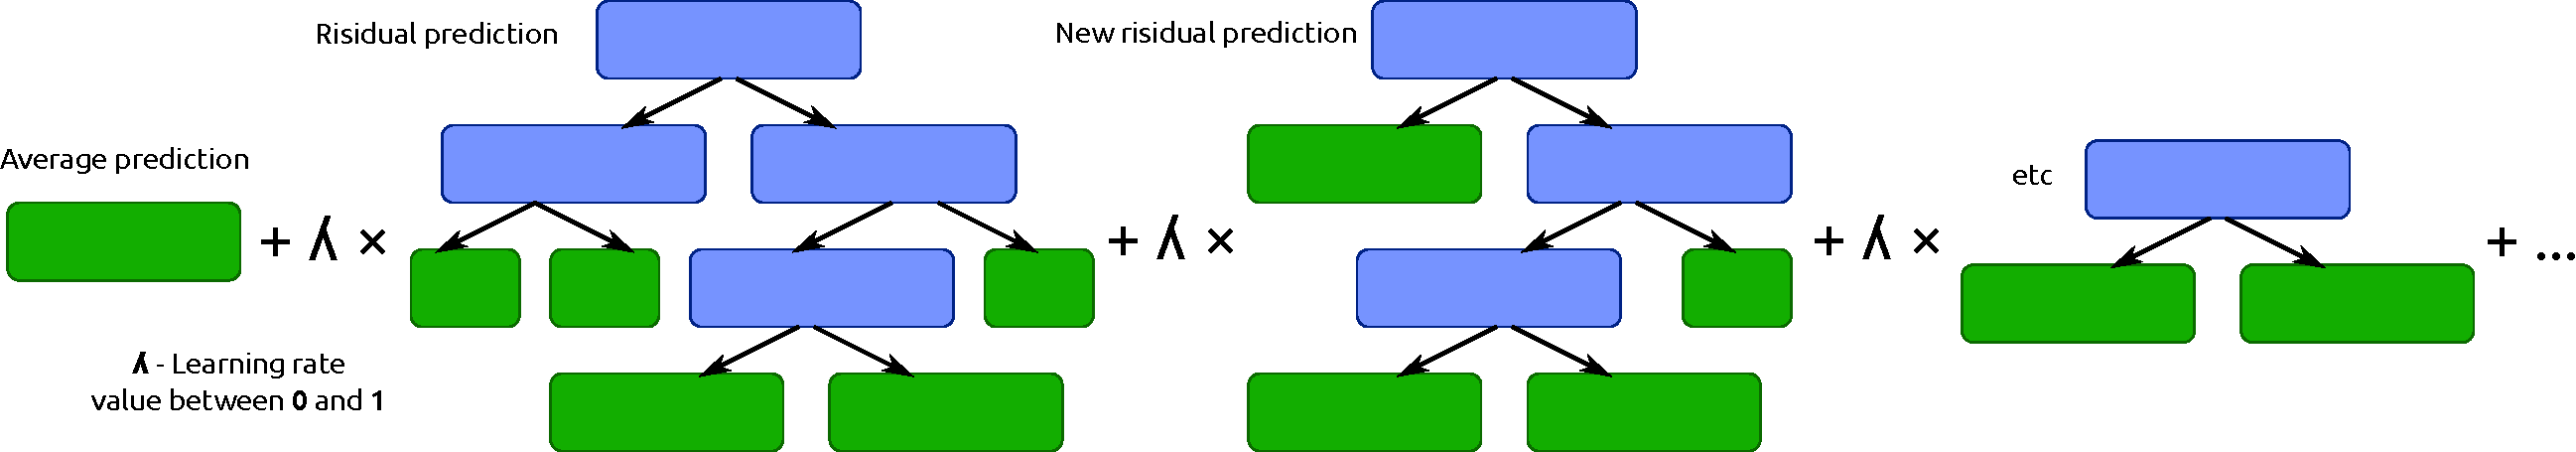
\includegraphics[width=1\linewidth]{images/boost/boosting_scheme.pdf}
    \caption{Gradient boosting scheme}
    \label{fig:boosting_scheme}
\end{figure}

On the other hand, Gradient Boosting takes a sequential approach to ensemble learning. Unlike Random Forests, which build trees independently, Gradient Boosting iteratively trains decision trees to correct the errors of their predecessors, as depicted in Fig.~\ref{fig:boosting_scheme}. By minimizing a loss function through a gradient descent-like optimization, Gradient Boosting gradually improves the accuracy of its predictions. This iterative correction process enables Gradient Boosting to adapt more effectively to the data, often outperforming other tree-based ensemble methods like Random Forests in terms of predictive accuracy~\cite{natekin2013gradient}. Variants like XGBoost, LightGBM, and CatBoost have emerged, focusing on enhancing speed and accuracy of this ensemble technique~\cite{bentejac2021comparative}.

% \subsubsection{Gradient Boosting in Optical Communication Systems}

Gradient Boosting has garnered attention as a promising equalization technique for optical communication systems due to its adaptability and capability to model complex input-output relationships \cite{Chen:2016:XST:2939672.2939785,natekin2013gradient,friedman2002stochastic,bentejac2021comparative}. One of its notable advantages is its robustness to overfitting, achieved through techniques like shrinkage, regularization, and early stopping. Furthermore, the inherent parallelizability of Gradient Boosting allows for efficient implementations on modern hardware architectures, including multi-core CPUs, GPUs, and even FPGAs \cite{alcolea2021fpga}, thus offering low-latency and power-efficient solutions crucial for real-time applications in optical communication systems.

In this part, we delve into the application of
% Gradient Boosting
\acrshort{gb}
as a novel equalization technique in optical communication systems. We aim to explore its potential to surpass the performance of traditional equalization methods, focusing on increasing predictive performance while simultaneously reducing the computational complexity of the equalization process. This innovative approach positions Gradient Boosting as a promising candidate for equalization tasks in optical communication systems, opening avenues for future advancements in the field.

\subsection{Theory of Gradient Boosting}

\acrfull{gb} builds a series of weak learners, usually decision trees, and iteratively refines the model by focusing on the areas where the previous models performed poorly. 

The algorithm starts with an initial model, \( F_0(x) \), which could be as simple as predicting the mean (for regression) or the majority class (for classification) for all instances in the dataset.

\begin{equation}
    F_0(x) = \arg\min_{\gamma} \sum_{i=1}^N L(y_i, \gamma) {,}
\end{equation}
where: \( N \) is the number of training instances,
\( L \) is the loss function,
\( y_i \) is the true label of the \( i \)-th instance,
\( \gamma \) is a constant.


The algorithm then enters a loop, for \( m = 1 \) to \( M \) (where \( M \) is the number of boosting rounds), where in each round it:
\begin{enumerate}
    \item Computes the pseudo-residuals, which are the gradients of the loss function with respect to the predicted values of the previous model, \( F_{m-1}(x) \):

\begin{equation}
r_{im} = -\left[\frac{\partial L(y_i, F(x_i))}{\partial F(x_i)}\right]_{F(x)=F_{m-1}(x)}
\end{equation}

    \item Fits a weak learner, \( h_m(x) \), to the pseudo-residuals, \( r_{im} \).

    \item Computes the optimal step size, \( \alpha_m \), that minimizes the loss function when \( h_m(x) \) is added to the current model:

\begin{equation}
\alpha_m = \arg\min_{\alpha} \sum_{i=1}^N L(y_i, F_{m-1}(x_i) + \alpha h_m(x_i))
\end{equation}

    \item Updates the model:

\begin{equation}
F_m(x) = F_{m-1}(x) + \alpha_m h_m(x)
\end{equation}

\end{enumerate}

The final model is the sum of the initial model and the products of the step sizes and the weak learners from each round:

\begin{equation}
F_M(x) = F_0(x) + \sum_{m=1}^M \alpha_m h_m(x)
\end{equation}


Each weak learner, \( h_m(x) \), is typically a shallow decision tree, and the loss function, \( L \), could be any differentiable loss function such as Mean Squared Error for regression or Logarithmic Loss for classification. The step size, \( \alpha_m \), helps in controlling the contribution of each weak learner, aiding in reducing overfitting and improving the model's generalization capability.

\subsubsection{Loss Functions}

Loss functions measure the difference between the predicted values and the true values. In Gradient Boosting, differentiable loss functions are used. The two common ones are \Gls{mse} (for regression) and Logistic Loss (for binary classification).

The loss function for \gls{mse} is given by:
\begin{equation}
L(y, F(x)) = \frac{1}{N} \sum_{i=1}^N (y_i - F(x_i))^2
\end{equation}

Taking the derivative with respect to \( F(x_i) \), we get:
\begin{equation}
\frac{\partial L(y, F(x))}{\partial F(x_i)} = -2(y_i - F(x_i))
\end{equation}

The loss function for Logistic Loss is given by:
\begin{equation}
L(y, F(x)) = - \frac{1}{N} \sum_{i=1}^N [ y_i \log(F(x_i)) + (1-y_i) \log(1-F(x_i)) ]
\end{equation}

Taking the derivative with respect to \( F(x_i) \), we get:
\begin{equation}
\frac{\partial L(y, F(x))}{\partial F(x_i)} = \frac{F(x_i) - y_i}{F(x_i)(1 - F(x_i))}
\end{equation}

In these formulas: \( N \) is the number of samples, \( y_i \) is the true label of the \( i \)-th instance, \( F(x_i) \) is the predicted value for the \( i \)-th instance.

For \gls{mse}, the derivative is straightforward and results in a simple expression involving the difference between the actual and predicted values.
For Logistic Loss, the derivative involves the quotient rule, and the expression relates the difference between the predicted probability and the actual label, normalized by the product of the predicted probability and its complement.


\subsubsection{Regularization}

Regularization is a technique used to prevent overfitting by adding a penalty on the complexity of the model. In Gradient Boosting, regularization can be achieved through various means:

\begin{enumerate}
    \item \textbf{Shrinkage (Learning Rate)}: 
    A small learning rate (also known as shrinkage) can be used to reduce the step size at each boosting step, making the boosting process more conservative.
    \[ F_m(x) = F_{m-1}(x) + \nu \cdot \alpha_m h_m(x) \]
    where \( \nu \) is the learning rate, \( 0 < \nu \leq 1 \).

    \item \textbf{Tree Complexity}:
    The complexity of the individual trees can be controlled by setting a maximum depth, minimum samples per leaf, or other similar parameters.

    \item \textbf{L1 (Lasso) and L2 (Ridge) Regularization}:
    These regularization terms can be added to the loss function to penalize the coefficients of the features.
    \[ L_{\text{regularized}}(y, F(x)) = L(y, F(x)) + \lambda_1 \sum | \beta | + \lambda_2 \sum \beta^2 \]
    where \( \beta \) are the coefficients of the features, and \( \lambda_1 \) and \( \lambda_2 \) are the regularization parameters.
\end{enumerate}


\subsection{Methodology}


In this study, we introduce a novel approach to nonlinear equalization in optical communication systems by employing a \acrshort{gb} algorithm based on decision trees.
We used an optical channel model of standard single-mode fiber (SSFM) with erbium-doped fiber amplifiers (EDFAs). The signal format is a 16-quadrature amplitude modulation (16-QAM) WDM with dual polarization and a symbol rate of $34.4\;\textrm{GBd}$. The pulse shaping employed a digital root-raised cosine (RRC) filter with a roll-off factor of $0.1$. The transmission distance varied between $10$, $15$, and $20$ spans of $80\;\textrm{km}$ each. The EDFA noise figure was set at $4.5\;\textrm{dB}$. The average signal power range was from $1$ to $8\;\textrm{dBm}$, but for training, we used power from $4\;\textrm{dBm}$ to $8 \textrm{dBm}$. The signal propagation through the fiber was represented by a generalized Manakov equation using the GPU-accelerated split-step Fourier method\cite{esf0_2023_7880552}. The fiber parameters included a wavelength of $\lambda = 1550\;\textrm{nm}$, a dispersion coefficient of $D = 16.8\;\textrm{ps}/(\textrm{nm} \cdot \textrm{km})$, and a nonlinear coefficient of $\gamma = 1.2\;\textrm{W}^{-1} \cdot \textrm{km}^{-1}$.

We generated around $10$ million datapoints for each specific average power and propagation distance. The dataset was then divided into training and test sets, with the test set comprising $1\%$ of the full dataset (about $100,000$ points).

In the dataset used for training, the input consists of values of the received points for the x-polarization, for which we aim to predict the nonlinear shift. To account for the neighboring points' influence, we include five values of received points to the right and left of the central point (neighbors in the sequence of points). Since we utilize two polarizations, we also incorporate the central point for y-polarization (in the same position in the sequence as for x-polarization) and its five neighboring points on both the left and right. As a result, a total of 22 complex points serve as input for the GB algorithm. The output represents the nonlinear shift (a complex number that must be added to accurately shift the point to its original position in the constellation) for the received point in the x-polarization.

The gradient boosting algorithm was implemented using the XGBoost library\cite{Chen:2016:XST:2939672.2939785} with GPU acceleration. The training process involved a large number of estimators, specifically $200,000$, which were chosen to test the idea of using decision trees but can be significantly reduced for a particular system. The maximum tree depth did not exceed $20$, the learning rate was set to $0.1$, and the $L_2$ and $L_1$ regularization parameters were both set to $1.0$.

\subsection{Complexity}
The complexity of prediction for gradient boosting can be expressed using the following formula:
$$
C(GB) = N_{trees} \cdot M \cdot N_{features}
$$
where $C(GB)$ represents the complexity of prediction for gradient boosting, $N_{trees}$ is the number of trees in the ensemble, $M$ is the maximum depth of each tree, $N_{features}$ is the number of features in the dataset.

This formula assumes that the complexity of each decision in the tree is constant and that the trees have a balanced structure. In practice, the trees might not be perfectly balanced, and the actual complexity could be somewhat lower. However, this formula provides a useful estimate for understanding the relationship between the main parameters of gradient boosting and its prediction complexity.

At first glance, it may appear that the overall complexity for our chosen set of parameters is excessively high. In this study, our primary goal is not to achieve cutting-edge complexity but rather to demonstrate the proof-of-concept. However, it is important to emphasize that each parameter contributing to complexity can be optimized to significantly reduce the overall complexity. Comprehensive information about feature importance allows us to manage input parameters (which can be further reduced) and to control the impact of each decision tree, thereby enabling the removal of unnecessary trees to enhance performance. Moreover, we can manually regulate the maximum depth of each tree, which, after optimization, can ultimately yield the desired performance.


\subsection{Results}

\begin{figure}[ht]
    \begin{minipage}[h]{0.49\linewidth}
    \center{
        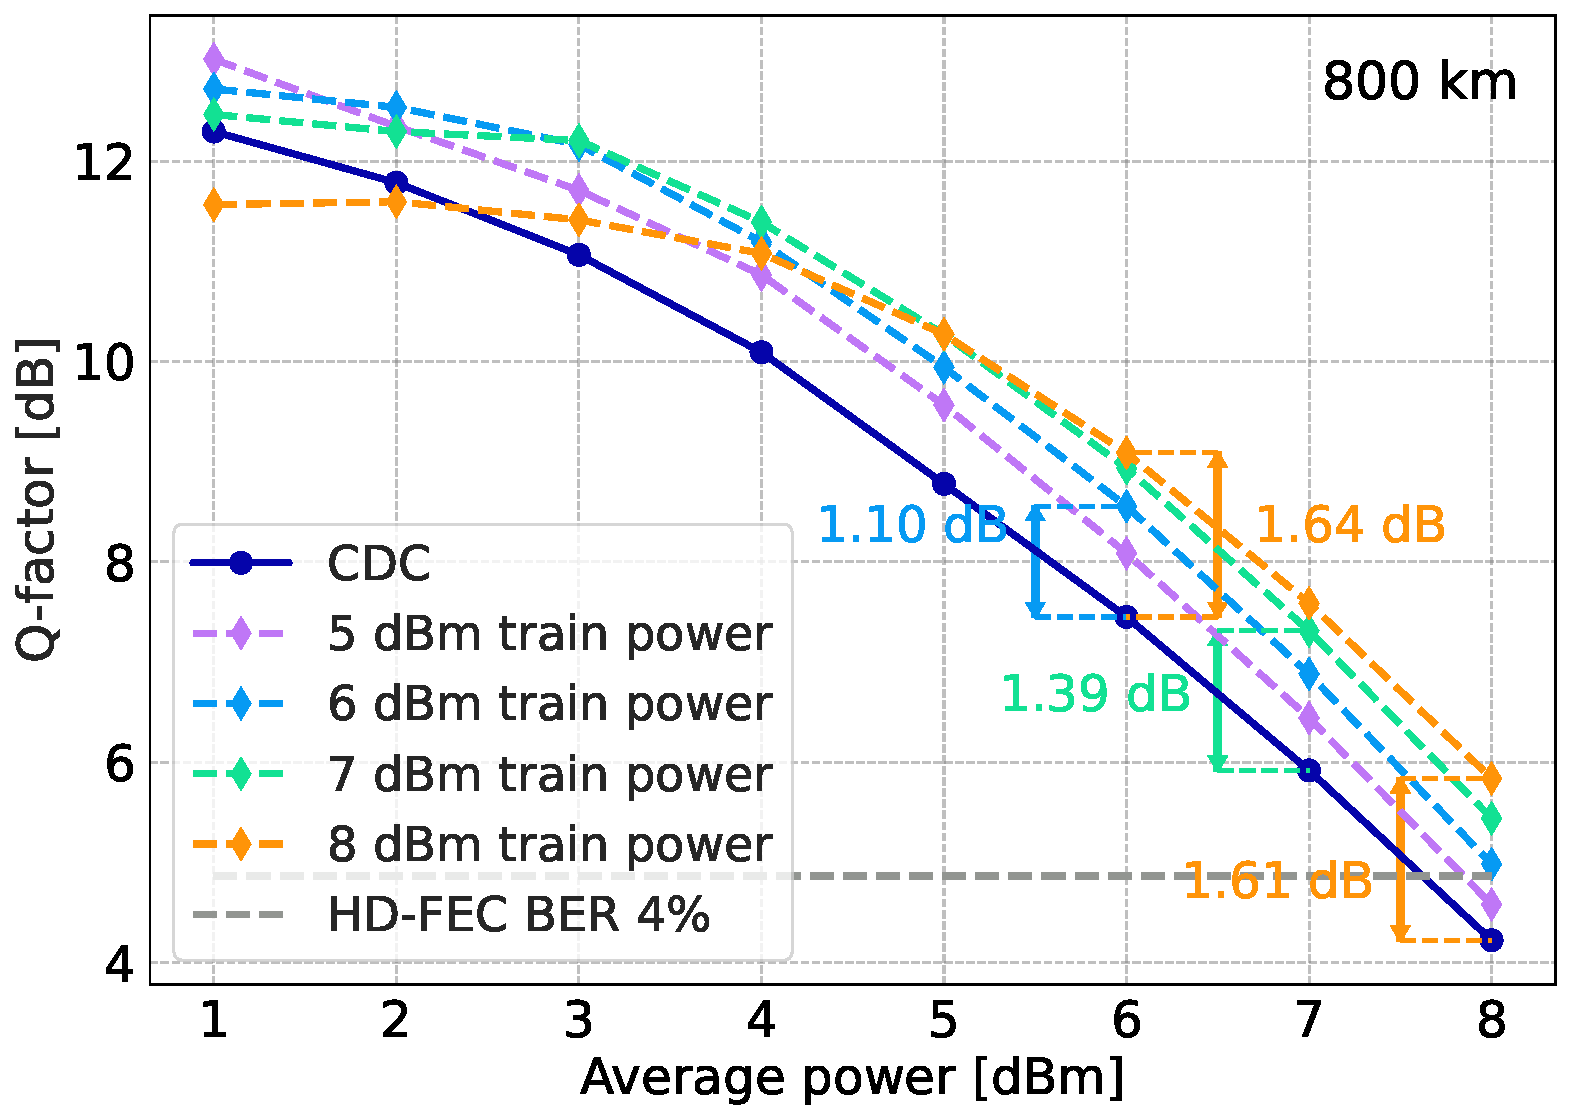
\includegraphics[width=1\linewidth]{images/boost/q_different_models_single_800.pdf} (a) \\
    }
    \end{minipage}
    \hfill
    \begin{minipage}[h]{0.49\linewidth}
    \center{
        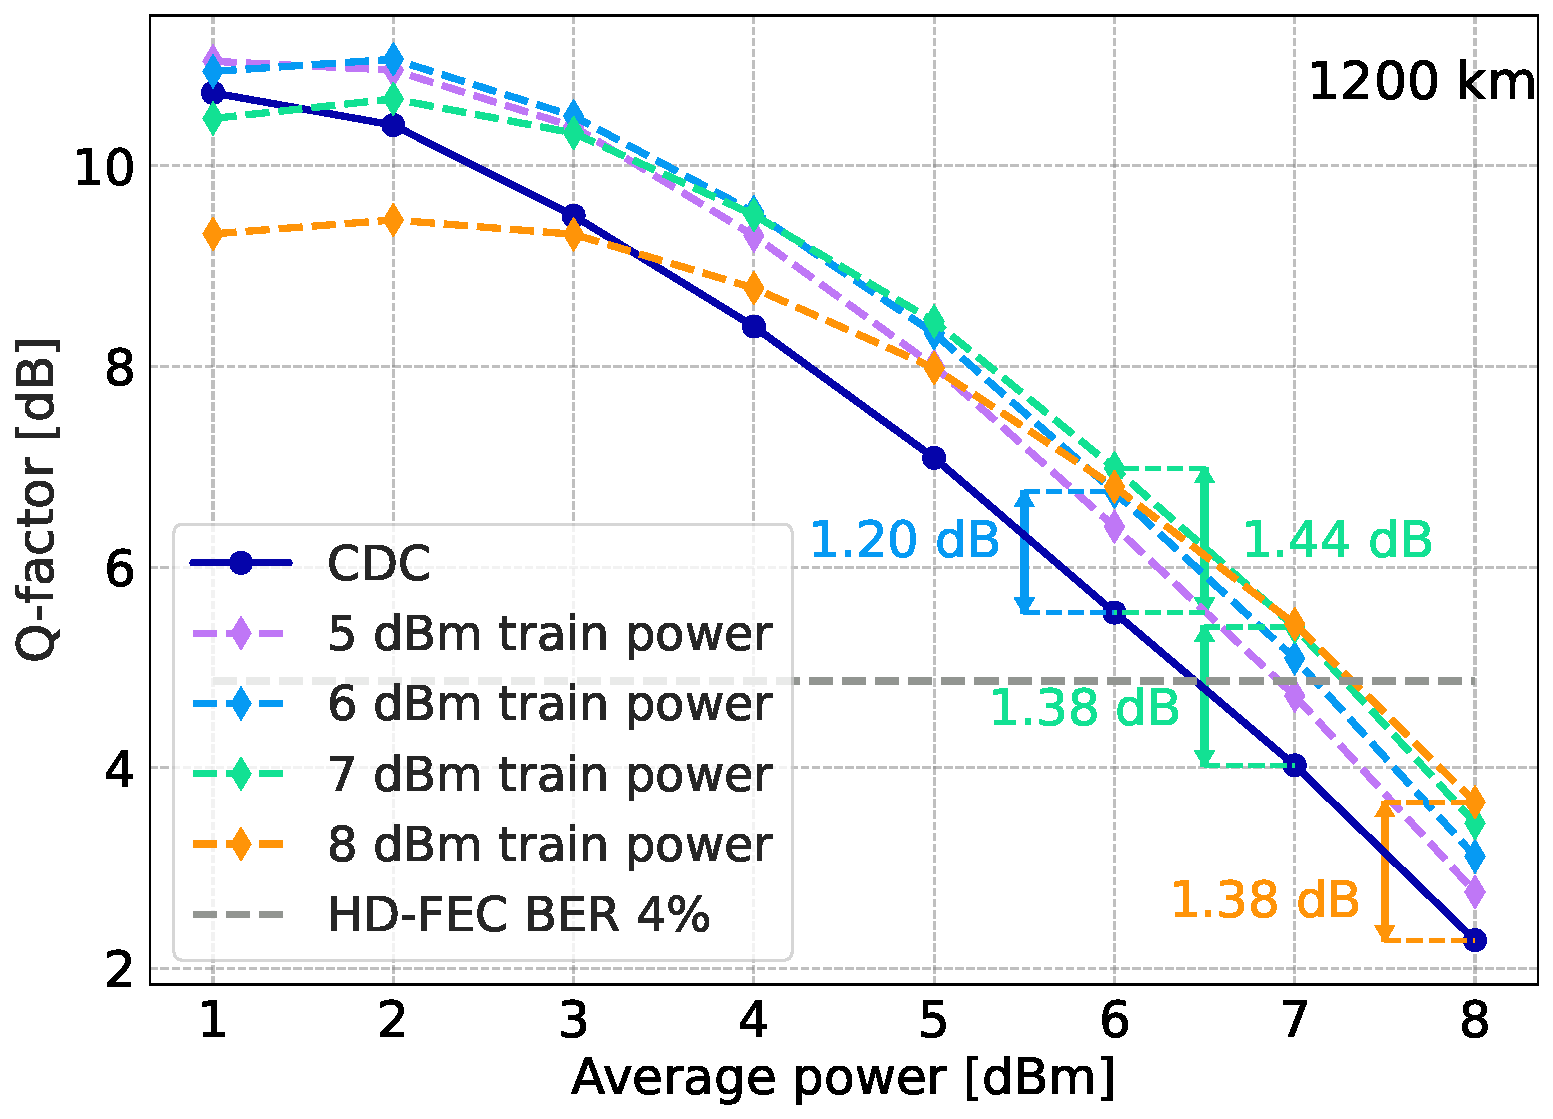
\includegraphics[width=1\linewidth]{images/boost/q_different_models_single_1200.pdf} (b) \\
    }
    \end{minipage}
    \vfill
    \center{
        \begin{minipage}[h]{0.49\linewidth}
        \center{
            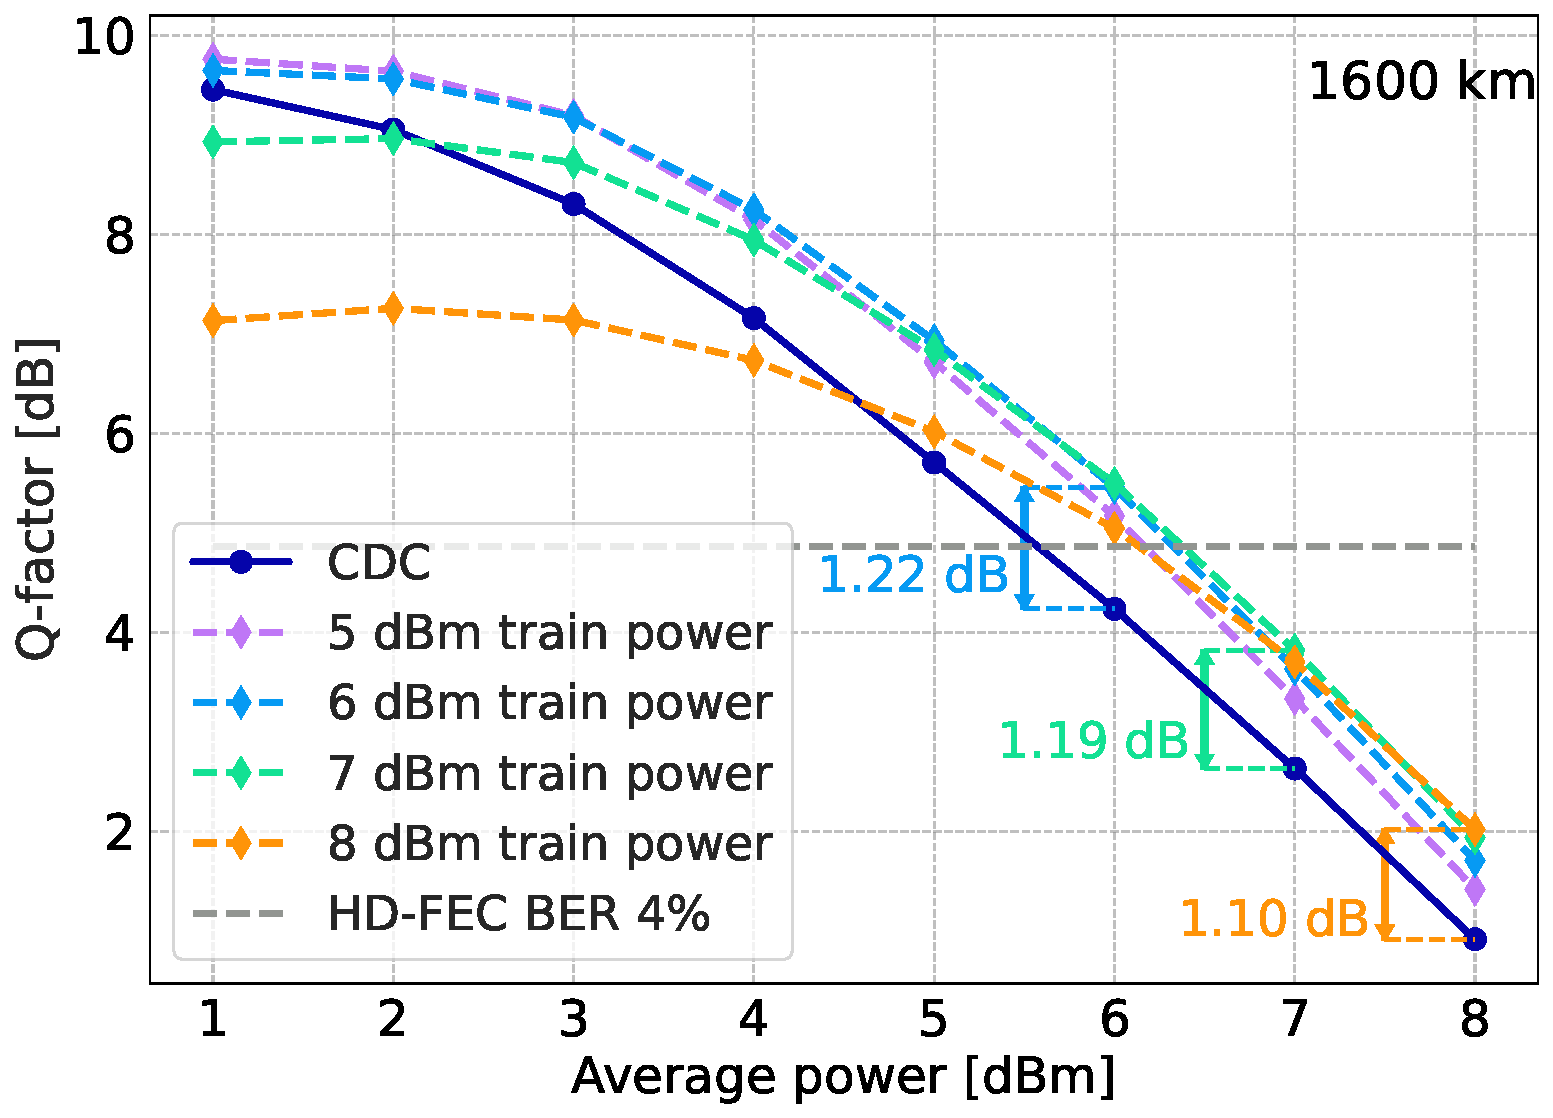
\includegraphics[width=1\linewidth]{images/boost/q_different_models_single_1600.pdf} (c) \\
        }
        \end{minipage}
    }
    \caption{Q-Factor performance after nonlinear equalization using GB trained at varying average signal power levels. Solid lines represent the system with CDC, and horizontal dashed lines indicate the HD-FEC threshold for a BER of 4\%. Total propagation distance of 800 km \textbf{(a)}, 1200 km \textbf{(b)} and 1600 km \textbf{(c)}.}
    \label{fig:boost_result}
\end{figure}


% \begin{figure*}[ht]
%    \centering
%     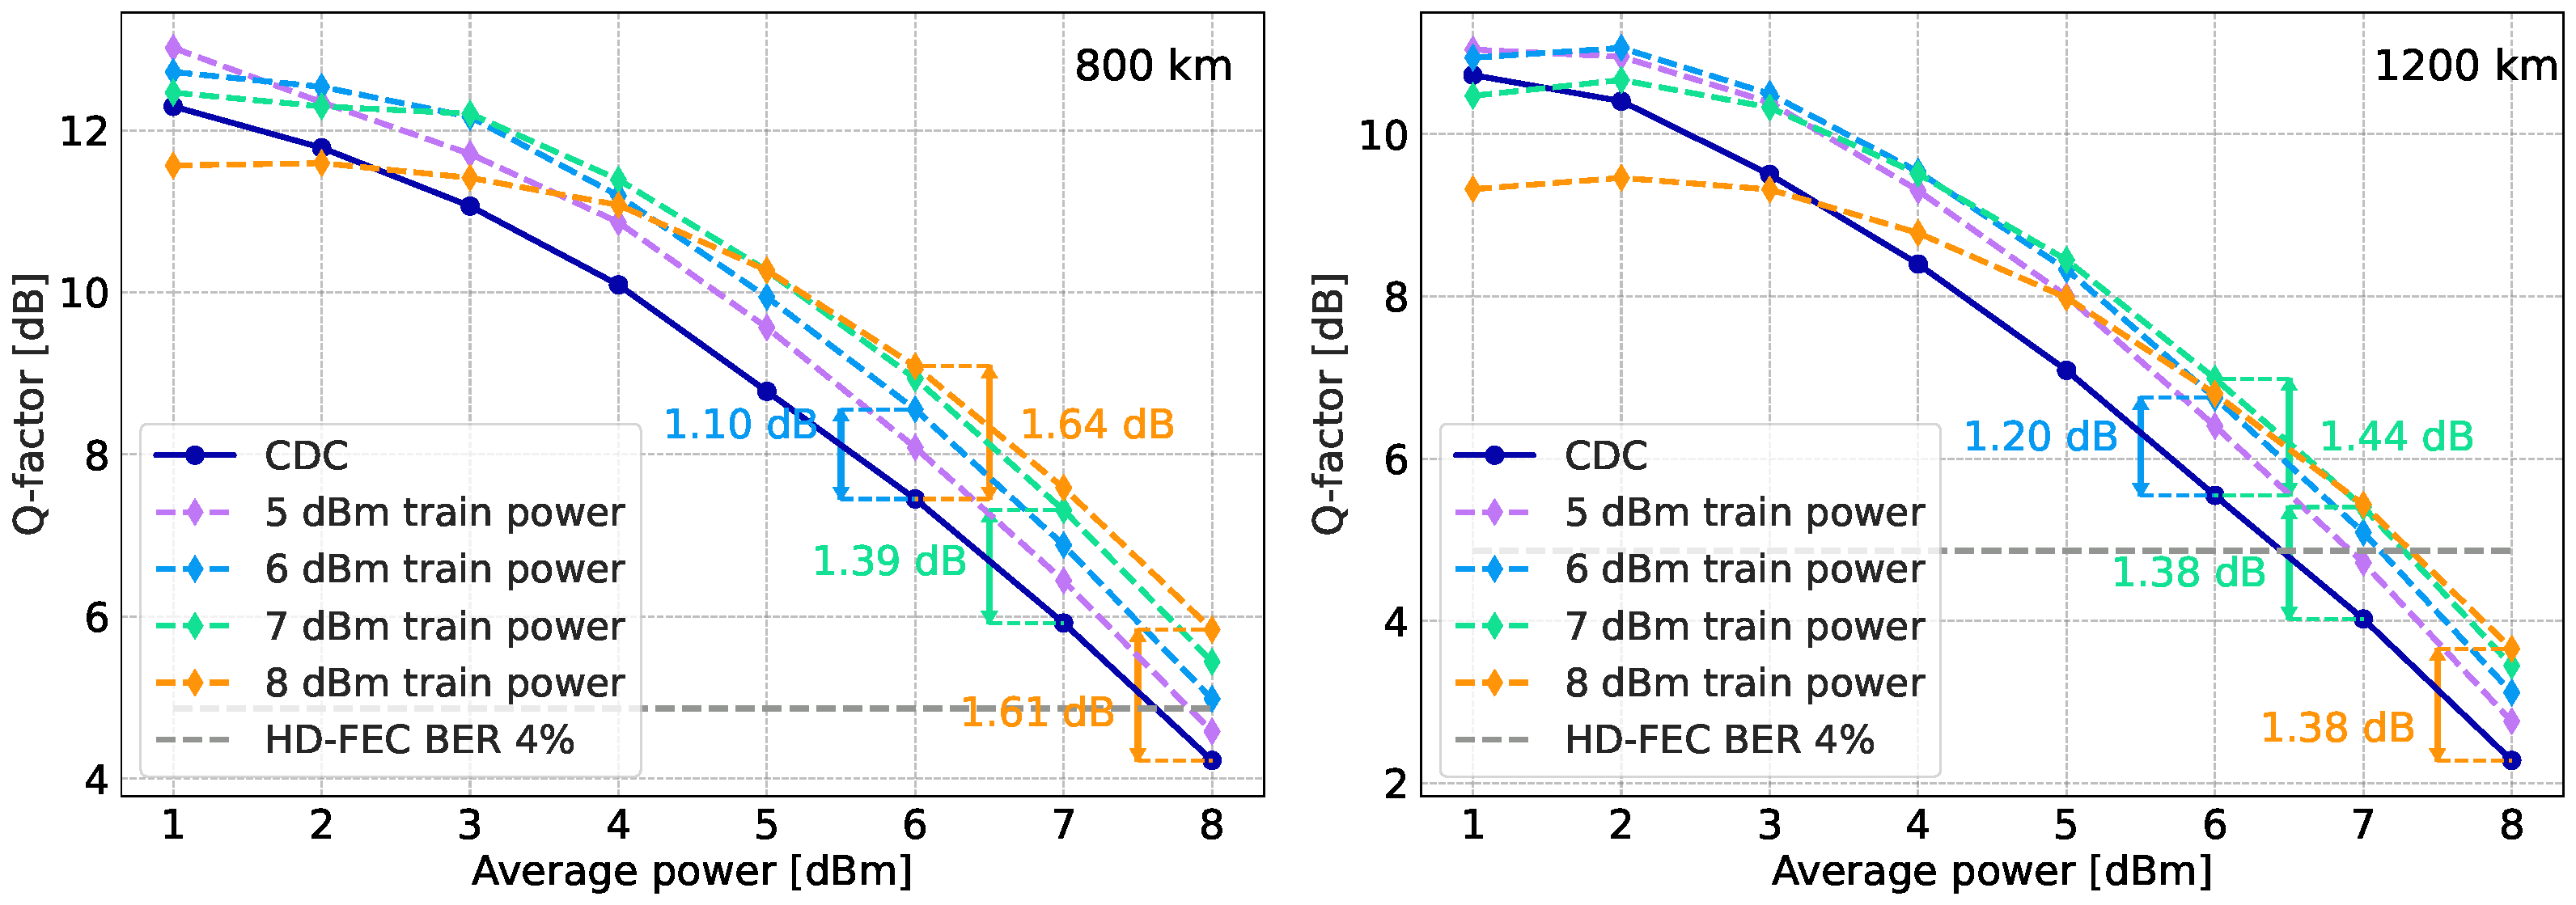
\includegraphics[width=1\linewidth]{images/boost/q_different_models_couple.pdf}
%     \caption{Q-Factor performance after nonlinear equalization using GB trained at varying average signal power levels. Solid lines represent the system with CDC, and horizontal dashed lines indicate the HD-FEC threshold for a BER of 4\%. Total propagation distance of 800 km \textbf{(left)}, and 1200 km \textbf{(right)}.}
%     \label{fig:fig1}
% \end{figure*}

% \begin{figure}[ht]
%    \centering
%         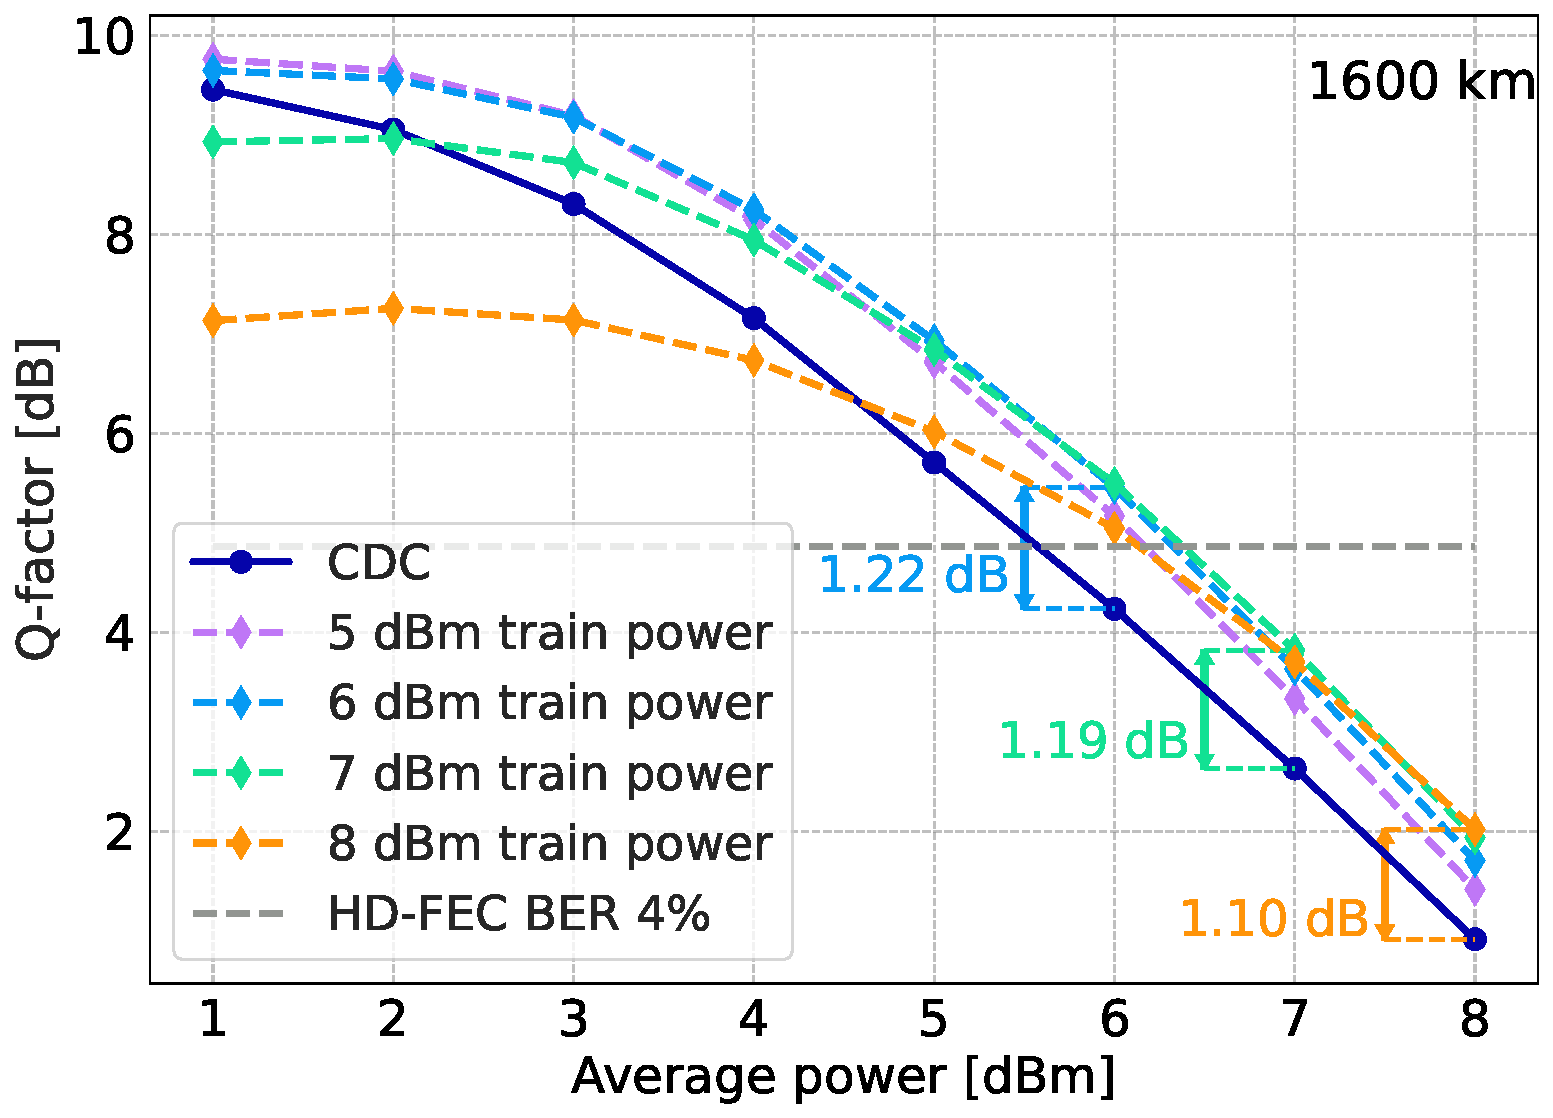
\includegraphics[width=0.5\linewidth]{images/boost/q_different_models_single.pdf}
%     \caption{Analogous to Fig.~\ref{fig:fig1}, Q-Factor performance for a total propagation distance of 1600 km, after nonlinear equalization using GB trained at different average signal power levels.}
%     \label{fig:fig2}
% \end{figure}


To demonstrate the potential of GB, we assessed the performance of various GB models across a range of propagation distances and diverse input signal average powers. The results were analyzed in terms of Q-factor improvement and the level of HD-FEC (Hard Decision Forward Error Correction), which represents a common error correction scheme used in optical communication systems. The target Bit Error Rate (BER) was set at $4\%$.

For all propagation distances, the GB models showed at least a $1\;\textrm{dB}$ improvement in Q-factor compared to the system with Chromatic Dispersion Compensation (CDC). Specifically, for a $1600\;\textrm{km}$ transmission distance (Fig.~\ref{fig:boost_result}c), the model trained on $8\;\textrm{dBm}$ signals exhibited a $1.10\;\textrm{dB}$ improvement in Q-factor for the same test power. The model trained on $7\;\textrm{dBm}$ signals displayed a $1.19\;\textrm{dB}$ improvement for the same test power, while the model trained on $6\;\textrm{dBm}$ signals showed a $1.22\;\textrm{dB}$ improvement. The $1.22\;\textrm{dB}$ Q-factor improvement for the $6\;\textrm{dBm}$ model allowed us to decrease the BER (increase the Q-factor) below (above) the HD-FEC level.

Interestingly, models trained on higher average power (and thus experiencing higher nonlinear distortions) exhibited good performance when applied to lower test power levels. However, their performance degraded for higher test power levels. This observation suggests that the GB algorithm can successfully mitigate nonlinear effects. This is particularly evident in Fig.~\ref{fig:boost_result}a for a propagation distance of $800\;\textrm{km}$. The model trained on $8\;\textrm{dBm}$ outperformed other models for power levels from $5\;\textrm{dBm}$ to $8\;\textrm{dBm}$, showing approximately $1.6\;\textrm{dB}$ improvement (specifically, $1.64\;\textrm{dB}$ for $6\;\textrm{dBm}$ test power and $1.61\;\textrm{dB}$ for $8\;\textrm{dBm}$ test power). For $8\;\textrm{dBm}$, the improved Q-factor surpassed the HD-FEC level. However, for lower signal powers, the model trained on $8\;\textrm{dBm}$ performed poorly, since these regimes are less influenced by nonlinear effects.

A similar pattern can be observed in Fig.~\ref{fig:boost_result}b for a propagation distance of $1200\;\textrm{km}$. In this case, the model trained on $7\;\textrm{dBm}$ showed significant improvement for a wide range of test signal powers (from $3\;\textrm{dBm}$ to $8\;\textrm{dBm}$). This finding indicates that the GB training power can be optimized for specific power ranges in which the system operates. The wide range of applicability allows for the development of a universal equalizer based on GB, which does not require retraining for different power levels (subject to the constraints of the working regime for GB).


\subsection{Conclusion}
In conclusion, this study has demonstrated the potential of gradient boosting as a novel equalization technique in optical communication systems, offering better predictive performance with the possibility of reduced complexity compared to traditional methods. This innovative approach may pave the way for advancements in the field and enhance the efficiency of modern telecommunication networks.

Future research should focus on optimizing the complexity-performance trade-off, investigating real-world robustness, and exploring hardware acceleration opportunities. Developing a universal equalizer based on gradient boosting could further expand the applicability of this technique in optical communication systems.